\chapter{Event selection}
\label{event_selection}
This chapter describes in detail the event selection criteria for the analyses, and how they were chosen. It starts by introducing the backgrounds that each of selection criterion is trying to reduce in order to get a higher ratio of number of signal events to background events, leading to a better sensitivity for the search. This is followed by the procedure for arriving at the best possible set of cuts.

\section{H125 analysis signature and backgrounds}
\label{h125_evt_selec}
The signature of the \hmue analysis final state consists of a muon that comes promptly from the Higgs and has a hard \pt spectrum, along with a softer electron that comes from the tau lepton, and missing transverse momentum from the tau decay. It is interesting to note that the signature is similar to the $\text{h} \to \Pgt_{\Pgm}\Pgt_{\Pe}$ decay that is allowed by the SM and since been observed, but with significant kinematic differences. In \hmue decay the $\Pgm$ comes directly from the Higgs resulting in its $\pt$ spectrum peaking and spreading out to much higher values. Also there are fewer neutrinos in \hmue, coming from the decay of the single $\Pgt$. The decay products of this highly boosted tau are closely aligned, leading to a narrow separation between the $\Pe$ and the \ptvecmiss in the azimuthal plane. The same is not true in the $\text{h} \to \Pgt_{\Pgm}\Pgt_{\Pe}$ decays. These differences are illustrated pictorially in Fig.~\ref{fig:htt_v_lfv}.

\begin{figure*}
\begin{center}
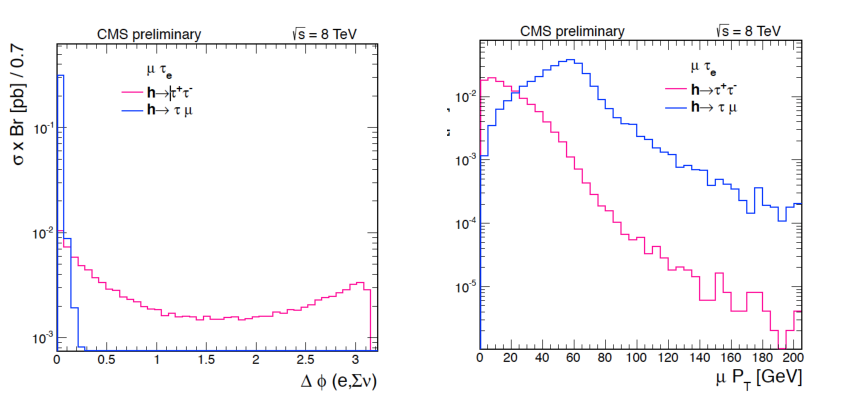
\includegraphics[width=0.8\textwidth,keepaspectratio]{plots_and_figures/chapter5/htt_v_lfv.pdf}
\caption{Illustration of the differences in $\Pgm_{\pt}$ and $\dphiemet$ spectrums in $\hmue$ and $\text{h} \to \Pgt_{\Pgm}\Pgt_{\Pe}$ processes.}
\label{fig:htt_v_lfv}
\end{center}
\end{figure*}

The most dominant backgrounds consists of \ztt events coming from Drell-Yan production and \ttb production. In \ztt events, one $tau$ can decay to an $\Pe$ and the other to a $\Pgm$. This background peaks at lower values of $M_{col}$ than the signal events but there is significant overlap with the signal spectrum. In \ttb production, each of the top quarks can decay into a bottom and a \PW with the \PW bosons then decaying to a $\Pe$ and $\Pgm$. The other backgrounds are smaller and include (in no particular order) electroweak diboson production ($\PW\PW$, $\PW\cPZ$ and $\cPZ\cPZ$), Higgs boson allowed by the SM ($\PH \to \Pgt\Pgt,\PW\PW$), $\PW\gamma^{(*)}+\text{jets}$ ,single top production, \wjets events, $Z\to\ell\ell$ $(\ell = \Pe, \Pgm)+\text{jets}$ and QCD multijet backgrounds. These backgrounds are described in more detail, along with there estimation and validation techniques in section~\ref{bg_val}.        


\subsection{Baseline selection and categorization}
\label{h125_evt_sel_bkg}

\subsection{Cut Based Selection}
\label{h125_cb_sel}

\subsection{BDT Based Selection}
\label{h125_bdt_Sel}

\subsubsection{Boosted Decision Trees}
\label{bdts}


\section{Heavy Higgs Analysis}
\label{hh_evt_selec}

\subsection{Backgrounds}
\label{hh_evt_sel_bkg}









% % uncomment the following lines,
% if using chapter-wise bibliography
%
% \bibliographystyle{ndnatbib}
% \bibliography{example}
